%-----------------------------------LICENSE------------------------------------%
%   This file is part of tikz_figures.                                         %
%                                                                              %
%   tikz_figures is free software: you can redistribute it and/or              %
%   modify it it under the terms of the GNU General Public License as          %
%   published by the Free Software Foundation, either version 3 of the         %
%   License, or (at your option) any later version.                            %
%                                                                              %
%   tikz_figures is distributed in the hope that it will be useful,            %
%   but WITHOUT ANY WARRANTY; without even the implied warranty of             %
%   MERCHANTABILITY or FITNESS FOR A PARTICULAR PURPOSE.  See the              %
%   GNU General Public License for more details.                               %
%                                                                              %
%   You should have received a copy of the GNU General Public License along    %
%   with tikz_figures.  If not, see <https://www.gnu.org/licenses/>.           %
%------------------------------------------------------------------------------%

% Use the standalone class for displaying the tikz image on a small PDF.
\documentclass[crop, tikz]{standalone}

% Import the tikz package to use for the drawing.
\usepackage{tikz}

% Tikz packages used.
\usetikzlibrary{decorations.markings, arrows.meta}

% Begin the document.
\begin{document}

    % Draw the figure.
    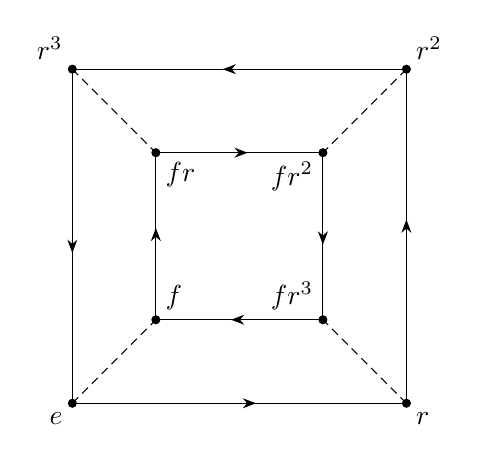
\begin{tikzpicture}[%
        ->-/.style = {%
            decoration = {%
                markings,
                mark = at position 0.55 with \arrow{Stealth}
            },
            postaction = {decorate}
        }
    ]

        % Coordinates for the outer square.
        \coordinate (e) at (225.0:3.0);
        \coordinate (r) at (315.0:3.0);
        \coordinate (r2) at (45.00:3.0);
        \coordinate (r3) at (135.0:3.0);

        % Coordinates for inner square.
        \coordinate (fr2) at (45.00:1.5);
        \coordinate (fr) at (135.0:1.5);
        \coordinate (f) at (225.0:1.5);
        \coordinate (fr3) at (315.0:1.5);

        % Dots for the coordinates.
        \foreach\x in {e, r, r2, r3, f, fr, fr2, fr3}{%
            \draw[fill = black] (\x) circle (0.05);
        }

        % Solid arrows for rotations.
        \draw[->-] (e) to (r);
        \draw[->-] (r) to (r2);
        \draw[->-] (r2) to (r3);
        \draw[->-] (r3) to (e);
        \draw[->-] (f) to (fr);
        \draw[->-] (fr) to (fr2);
        \draw[->-] (fr2) to (fr3);
        \draw[->-] (fr3) to (f);

        % Dashed arrows for reflections.
        \draw[densely dashed] (e) to (f);
        \draw[densely dashed] (r) to (fr3);
        \draw[densely dashed] (r2) to (fr2);
        \draw[densely dashed] (r3) to (fr);

        % Label the points.
        \node at (e) [below left] {$e$};
        \node at (r) [below right] {$r$};
        \node at (r2) [above right] {$r^{2}$};
        \node at (r3) [above left] {$r^{3}$};
        \node at (f) [above right] {$f$};
        \node at (fr3) [above left] {$fr^{3}$};
        \node at (fr2) [below left] {$fr^{2}$};
        \node at (fr) [below right] {$fr$};
    \end{tikzpicture}
\end{document}
